% Diagrama C — espaço de subconjuntos para três canais: cadeia prefixada
% (SLACGS) versus enumeração exaustiva (CoInfoSim).
\documentclass[tikz,border=6pt]{standalone}
% Preâmbulo compartilhado dos diagramas conceituais do relatório CoInfoSim.
% Compilação: xelatex (determinística; nenhum dado experimental é usado).
\usepackage{fontspec}
\setmainfont{Liberation Sans}
\setsansfont{Liberation Sans}
\usepackage{amsmath}
\usepackage{bm}
\usepackage{tikz}
\usetikzlibrary{arrows.meta,positioning,calc,fit,backgrounds,decorations.pathreplacing,matrix,patterns}
\definecolor{CoinAccent}{RGB}{25,80,140}
\definecolor{CoinAccentDark}{RGB}{18,55,95}
\definecolor{CoinAccentPale}{RGB}{237,242,248}
\definecolor{CoinGray}{RGB}{95,95,95}
\definecolor{CoinGrayPale}{RGB}{246,246,246}
\definecolor{CoinWin}{RGB}{76,140,90}    % verde discreto (vitória)
\definecolor{CoinLose}{RGB}{182,88,79}   % vermelho discreto (derrota)
\tikzset{
  bloco/.style={draw=CoinAccentDark, fill=CoinAccentPale, rounded corners=1.2pt,
                align=center, font=\small, inner sep=4pt, minimum height=7mm},
  bloconeutro/.style={draw=CoinGray, fill=CoinGrayPale, rounded corners=1.2pt,
                align=center, font=\small, inner sep=4pt, minimum height=7mm},
  blocoreal/.style={draw=CoinAccentDark, fill=white, rounded corners=1.2pt,
                align=center, font=\small, inner sep=4pt, minimum height=7mm},
  seta/.style={-{Stealth[length=2.4mm]}, thick, CoinAccentDark},
  setacinza/.style={-{Stealth[length=2.4mm]}, thick, CoinGray},
  rotulo/.style={font=\footnotesize\itshape, text=CoinGray, align=center},
}

\begin{document}
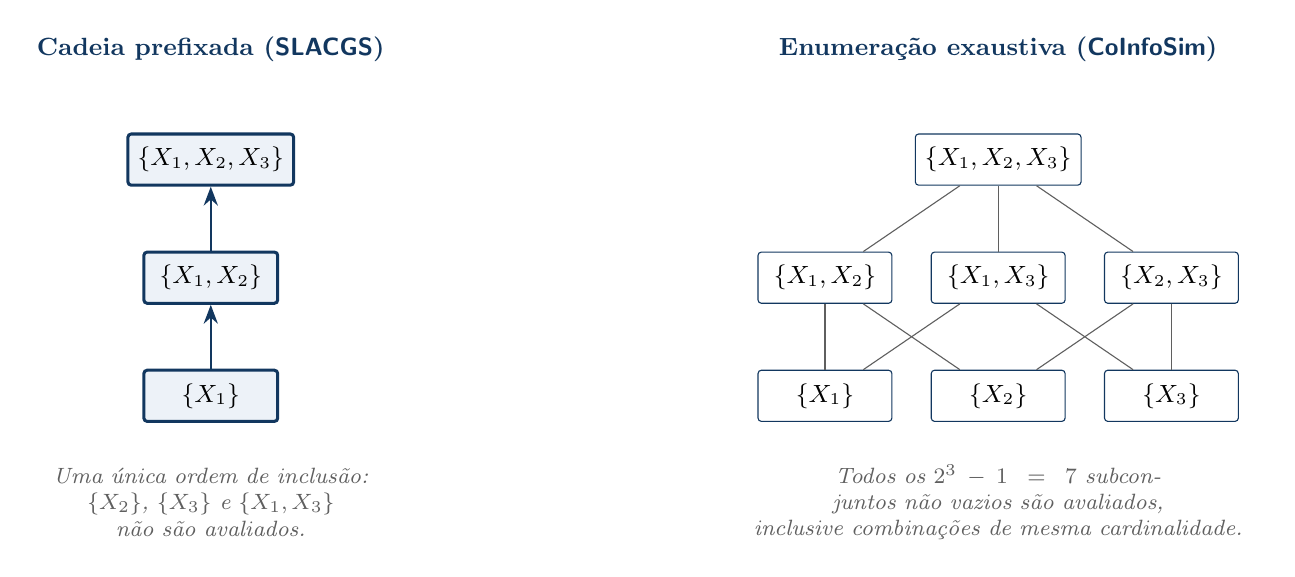
\begin{tikzpicture}[node distance=6mm]
  \tikzset{sub/.style={draw=CoinAccentDark, fill=white, rounded corners=1.2pt,
           font=\small, inner sep=3.5pt, minimum width=17mm, minimum height=6.5mm, align=center},
           subpref/.style={sub, fill=CoinAccentPale, line width=1.1pt}}

  % Painel esquerdo: cadeia prefixada
  \begin{scope}[xshift=-4.9cm]
    \node[font=\small\bfseries, text=CoinAccentDark] at (0,4.4) {Cadeia prefixada (\textsf{SLACGS})};
    \node[subpref] (a1) at (0,0)   {$\{X_1\}$};
    \node[subpref] (a2) at (0,1.5) {$\{X_1,X_2\}$};
    \node[subpref] (a3) at (0,3.0) {$\{X_1,X_2,X_3\}$};
    \draw[seta] (a1) -- (a2);
    \draw[seta] (a2) -- (a3);
    \node[rotulo, text width=4.3cm] at (0,-1.35)
      {Uma única ordem de inclusão:\\$\{X_2\}$, $\{X_3\}$ e $\{X_1,X_3\}$\\não são avaliados.};
  \end{scope}

  % Painel direito: reticulado completo
  \begin{scope}[xshift=2.9cm]
    \node[font=\small\bfseries, text=CoinAccentDark] at (2.2,4.4) {Enumeração exaustiva (\textsf{CoInfoSim})};
    % nível 1
    \node[sub] (s1) at (0,0)   {$\{X_1\}$};
    \node[sub] (s2) at (2.2,0) {$\{X_2\}$};
    \node[sub] (s3) at (4.4,0) {$\{X_3\}$};
    % nível 2
    \node[sub] (s12) at (0,1.5)   {$\{X_1,X_2\}$};
    \node[sub] (s13) at (2.2,1.5) {$\{X_1,X_3\}$};
    \node[sub] (s23) at (4.4,1.5) {$\{X_2,X_3\}$};
    % nível 3
    \node[sub] (s123) at (2.2,3.0) {$\{X_1,X_2,X_3\}$};
    % arestas de inclusão
    \foreach \a/\b in {s1/s12, s1/s13, s2/s12, s2/s23, s3/s13, s3/s23,
                       s12/s123, s13/s123, s23/s123}{
      \draw[CoinGray, thin] (\a) -- (\b);
    }
    \node[rotulo, text width=6.6cm] at (2.2,-1.35)
      {Todos os $2^{3}-1=7$ subconjuntos não vazios são avaliados,\\
       inclusive combinações de mesma cardinalidade.};
  \end{scope}
\end{tikzpicture}
\end{document}
